\documentclass{article}
\usepackage[UTF8]{ctex}
% Replace `letterpaper' with`a4paper' for UK/EU standard size
\usepackage[a4paper,top=2cm,bottom=2cm,left=3cm,right=3cm,marginparwidth=1.75cm]{geometry}

% Useful packages
\usepackage{amsmath}
\usepackage{graphicx}
\usepackage[colorlinks=true, allcolors=blue]{hyperref}
\usepackage{graphicx} %插入图片的宏包
\usepackage{float} %设置图片浮动位置的宏包
\usepackage{subfigure} %插入多图时用子图显示的宏包
\usepackage{parskip}
\usepackage{indentfirst} 
\setlength{\parindent}{2em}
\usepackage{hyperref}  
\usepackage{tikz}
\allowdisplaybreaks
\usepackage{multirow}

\title{基于微分思想与数值模拟的多波束海底测深布线模型}
%\author{}

\begin{document}
	\newcommand\degree{^\circ}
	\maketitle
	
	\begin{abstract}
		
	\end{abstract}
\tableofcontents
	
\section{问题背景重述}
\subsection{问题背景}
\subsection{问题重述}

\section{问题分析}
\subsection{问题一分析}
	在问题一中,海底被假想为一个坡面,测量船沿着海底等深线方向探测,也即$\beta=90\degree$的方向进行测深。在本问题中,我们规定覆盖宽度$w$投影到水平面上。首先,在已知坡度$\alpha$、水深$D$和多波束换能器开角$\theta$的前提下,利用正弦定理等平面几何知识,可得到覆盖宽度$w$。再者,在进一步知道两条相邻侧线的距离$d$的情况下,可得重叠率$\eta$。最后,将具体的$alpha=1.5 \degree,\, D=70m,\,\theta=120\degree, \, \d=200 $ 代入我们建立的模型,即可得到表一结果。
	
\subsection{问题二分析}
	问题二是问题一的推广,问题一是问题二在$\beta=90\degree$时的特例。在问题二中,海底仍然被假想为一个坡面,但测量船的测量方向与海底坡面法向在水平面上的投影成一定的夹角$\beta$。我们仍规定覆盖宽度$w$投影到水平面上。首先,沿法向量在水平面上的投影、等深线以及竖直方向,我们建立了空间直角坐标系。其次,我们注意到多波束平面与海底坡面会形成一条交线,利用解析几何的知识,这条交线与水平面形成的线面角$\gamma$的大小只和$\alpha$与$\beta$有关。在确定了$\gamma$之后,第二问即可转化为第一问。最后,第二问要求在不同的$\beta$以及不同的测量船距海域中心点距离$L$的条件下计算覆盖宽度$w$,我们根据空间几何关系,由$\beta$和$L$计算出水深$D$,将$D$和$\beta$带入第一问建立的模型求解,可得表二结果。

\subsection{问题三分析}
	问题三建立在第二问所建立模型的基础上。第三问要求给出对某理想矩形海域全覆盖、且满足覆盖率要求的最优布线。首先,我们由第二问的模型,推断出在任何水深$D$的情况下,$\beta=90\degree$或者$\beta = 180\degree$的时候都有$w$取最大值。其次,我们基于贪心原则和积分中值定理的思想,认为在“充分利用”覆盖宽度的条件下才可能得到最短布线,且考虑到了斜线行驶很可能会引发角落处覆盖不全的难题,因此把可行域空间限制在测线平行于等深线的情况内。然后,在考虑平行等深线布线的情况下,以总测线长度为目标函数,以覆盖范围和重叠率为约束条件,可以建立最优化模型。最后,在测线条数$n=32~40$的情况下利用matlab分别找满足条件的布线最优解,在$n=34$时找到了最短路径,并给出了各条测线之间的重叠率。
	

\subsection{问题四分析}
	本题提供了早期进行单波束测量时留下的网格化离散水深数据,但要求进行连续测线的规划。本题需要将前三问建立的理想坡度下的模型应用于真实世界中凹凸不平的海域,且同时要进行多目标的优化。
	\par 首先,我们将海域深度数据可视化,发现该海域近似为一个马鞍面,起伏较大,无法直接套用理想坡度模型。其次,我们分析了题给的三个目标,并且根据地理测绘的实际需求,认为诸目标的优先次序从高到低应该是:提高覆盖面积(保证数据完整有效)、降低总长度(节省测量成本)、控制重叠率(降低冗余度)。
	\par 接着,我们基于类似有限差分的思想,利用最小二乘法,计算出网格上各点的局部坡度,并用法向量来表征局部坡度信息。我们通过K-means算法,综合考虑各个点的位置、水深和局部坡度法向量,将该区域剖分为多个坡度相近的矩形和梯形子区域。在剖分之后,我们利用图论算法,给出遍历这几个区域的可能顺序,并确定相邻区域的路线衔接点,也即各区域测线的起点和终点。
	\par 我们把每个子区域都转化为第三问的情况,把各子区域的海底视为理想的坡面,在每个子区域内部进行最优路线规划,在各子区域内尽可能减少路程和重叠率并增加覆盖面积,把各子区域路线连接起来得到总路线。然后,把待选的总测线运用于真实的海底中,通过数值积分的方式,测算路线长度、覆盖面积和高重叠率($\eta \ge$ 20$\%$)的路线长度。最后,通过综合评价的方式,选出多目标规划下的最优路线。


\section{模型假设}
\begin{enumerate}
	\item 覆盖宽度$w$指的是将坡度上的覆盖范围垂直投影到水平面后的宽度。
	\item 与波束在海中的传播速度相比,探测船的运动速度忽略不计,也即认为发射声波与接收回声的时候,探测船处于相同的位置。
	\item 探测船在海洋中摇晃所带来的精度损失忽略不计,一旦多波束换能器的开角$\theta$确定且探测船的位置与行驶方向确定,多波束在某位置的覆盖宽度就确定。
	\item 在规划布线时,测量船可以在目标海域内或目标海域外的任意一点开始或结束探测工作。
	\item 在第三问中,测量船绕到目标海域外行驶,或者沿边界处行驶时(比如掉头),我们假设测量船会\textbf{关闭}多波束换能器。我们把此段路程算入测线的总长度中,但认为探测面积为0,与其他部分测线的重叠率为0。
	\item 在第四问中,我们将目标海域分化为若干个子区域。我们假设测量船在测量完一个子区域之后,必须到达该子区域的其中一条边界,并且只能前往与该区域在此边界相交的下一个相邻区域。我们假设从上一个子区域的探测终点前往下一个相邻区域的探测起点的过程中测量船会\textbf{关闭}多波束换能器,我们不把此段路程算入测线总长度中,且认为探测面积为0,与其他部分测线重叠率为0。
\end{enumerate}


\section{符号申明}

\begin{table}[H]
	\centering
	\begin{tabular}{ll}
	\hline
	符号	&  含义\\ 
	\hline
	$\alpha$	&  		\\
	$\beta$		&  		\\
	$\gamma$	&  		\\
	$\theta$			&  		\\ 
	$\eta$			&  		\\ 
	$w$			&  		\\
	$d$			&  		\\ 
	$D$			&  		\\ 
	$L$			&  		\\ 
	
	\hline
	\end{tabular}
\end{table}

\section{模型建立与求解}
\subsection{问题一:沿等深线测深时的宽度与重叠率计算}
\subsubsection{利用正弦定理计算覆盖宽度w}
	\par 第一问的几何示意图如\ref{pro1Geo}所示。其中,S为测量船,$D=SP$为测量船所在位置的水深。$w=MN\cos\alpha$为测量宽度。
	
	\begin{figure}[H]
		\centering  %图片全局居中
		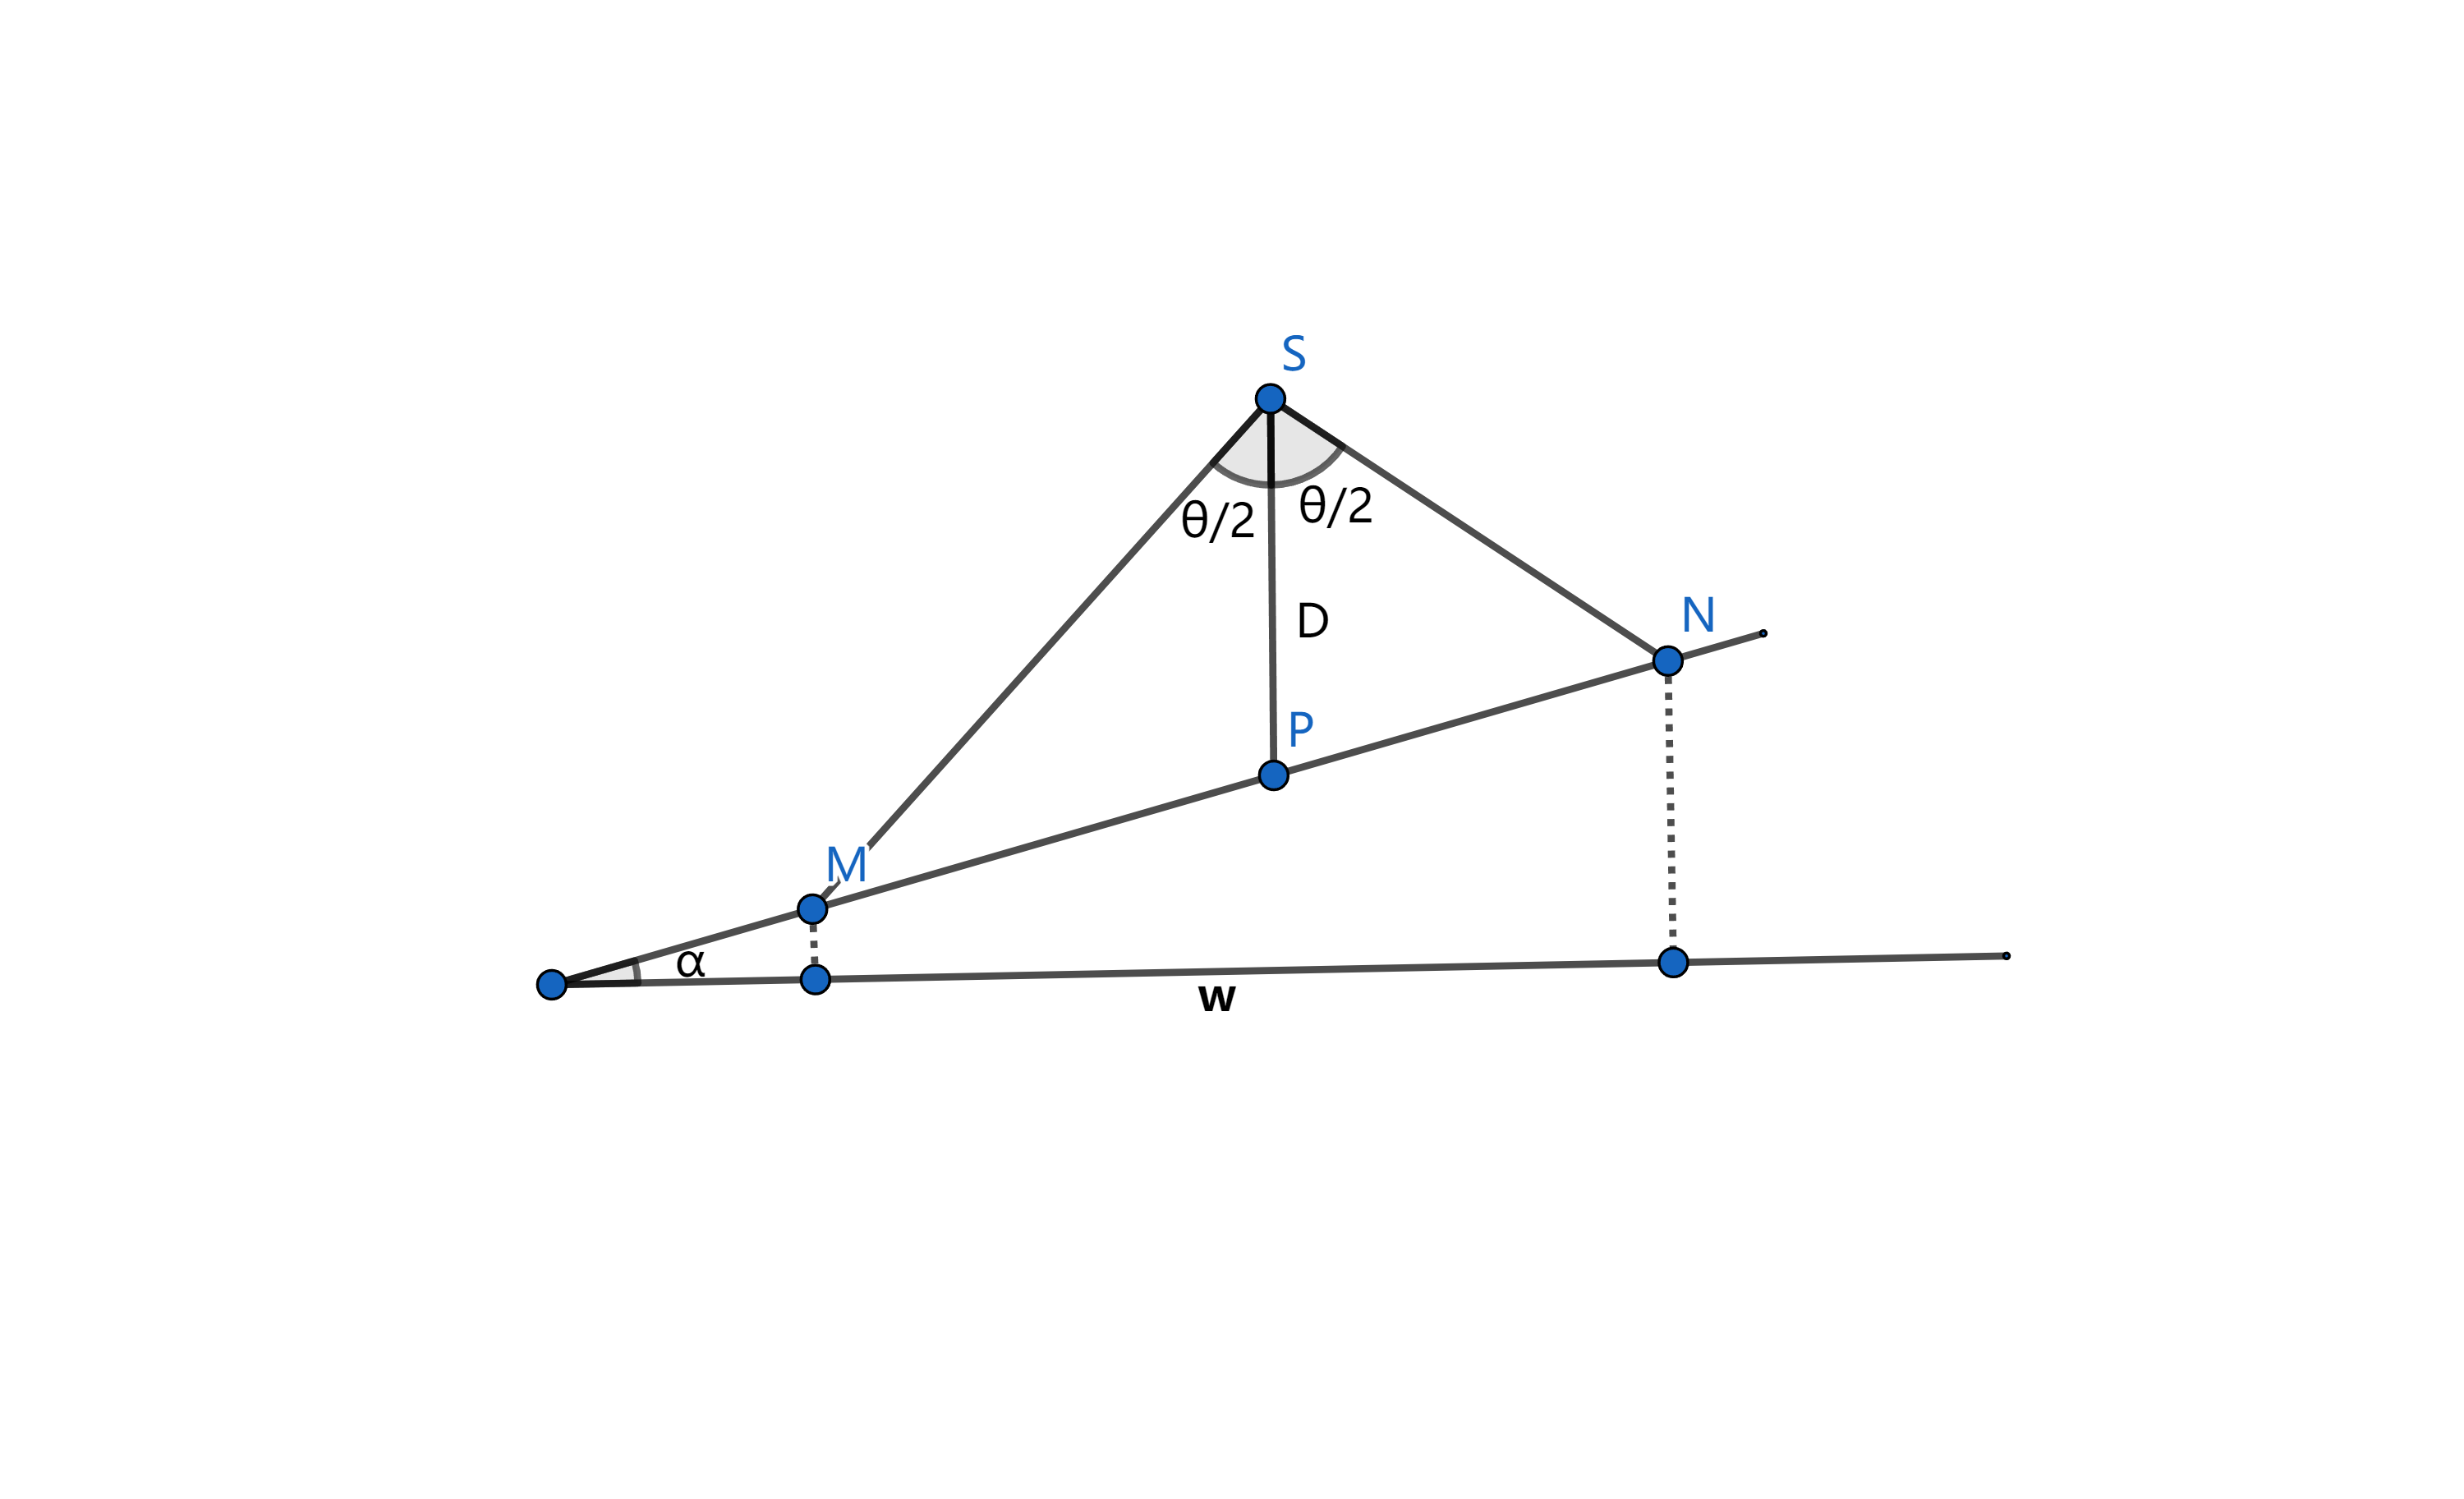
\includegraphics[width=0.95\textwidth]{问题一//问题一几何关系示意图}
		\caption{第一问覆盖宽度的几何关系示意图}
		\label{pro1Geo}
	\end{figure}
	\par 根据\textbf{正弦定理},我们分别在$\Delta MPS$和$\Delta NPS$中分别可以得到如下的关系
	
	\[
		\frac{MP}{\sin\frac{\theta}{2}} = \frac{D}{\sin(\frac{\pi-\theta}{2}-\alpha)}    
	\]
	\[
	\frac{NP}{\sin\frac{\theta}{2}} = \frac{D}{\sin(\frac{\pi-\theta}{2}+\alpha)}   \]
	

	\par 根据几何关系,我们可以得到:
	\begin{align}
		MN = MP + NP \label{eq1}  \\
		w = MN\cos\alpha  \label{eq2} 
	\end{align}
	
	\par 其中\eqref{eq1}与\eqref{eq2}是在第二问和第三问中依然成立的关系式,只不过其中的$\alpha$需要替换成$\gamma$(详后)。整理上述各关系式,我们求解得到:
	\begin{equation}
		w = w(D) = D\cos\alpha\left[\frac{\sin\frac{\theta}{2}}{\cos(\frac{\theta}{2}+\alpha)}  +  \frac{\sin\frac{\theta}{2}}{\cos(\frac{\theta}{2}-\alpha)}\right] \label{eq3}
	\end{equation}


\subsubsection{重叠率的计算公式推导}
	\par 下面我们推导重叠率的计算公式。重叠情况的示意图如图\ref{pro1Eta}所示:
		\begin{figure}[H]
		\centering  %图片全局居中
		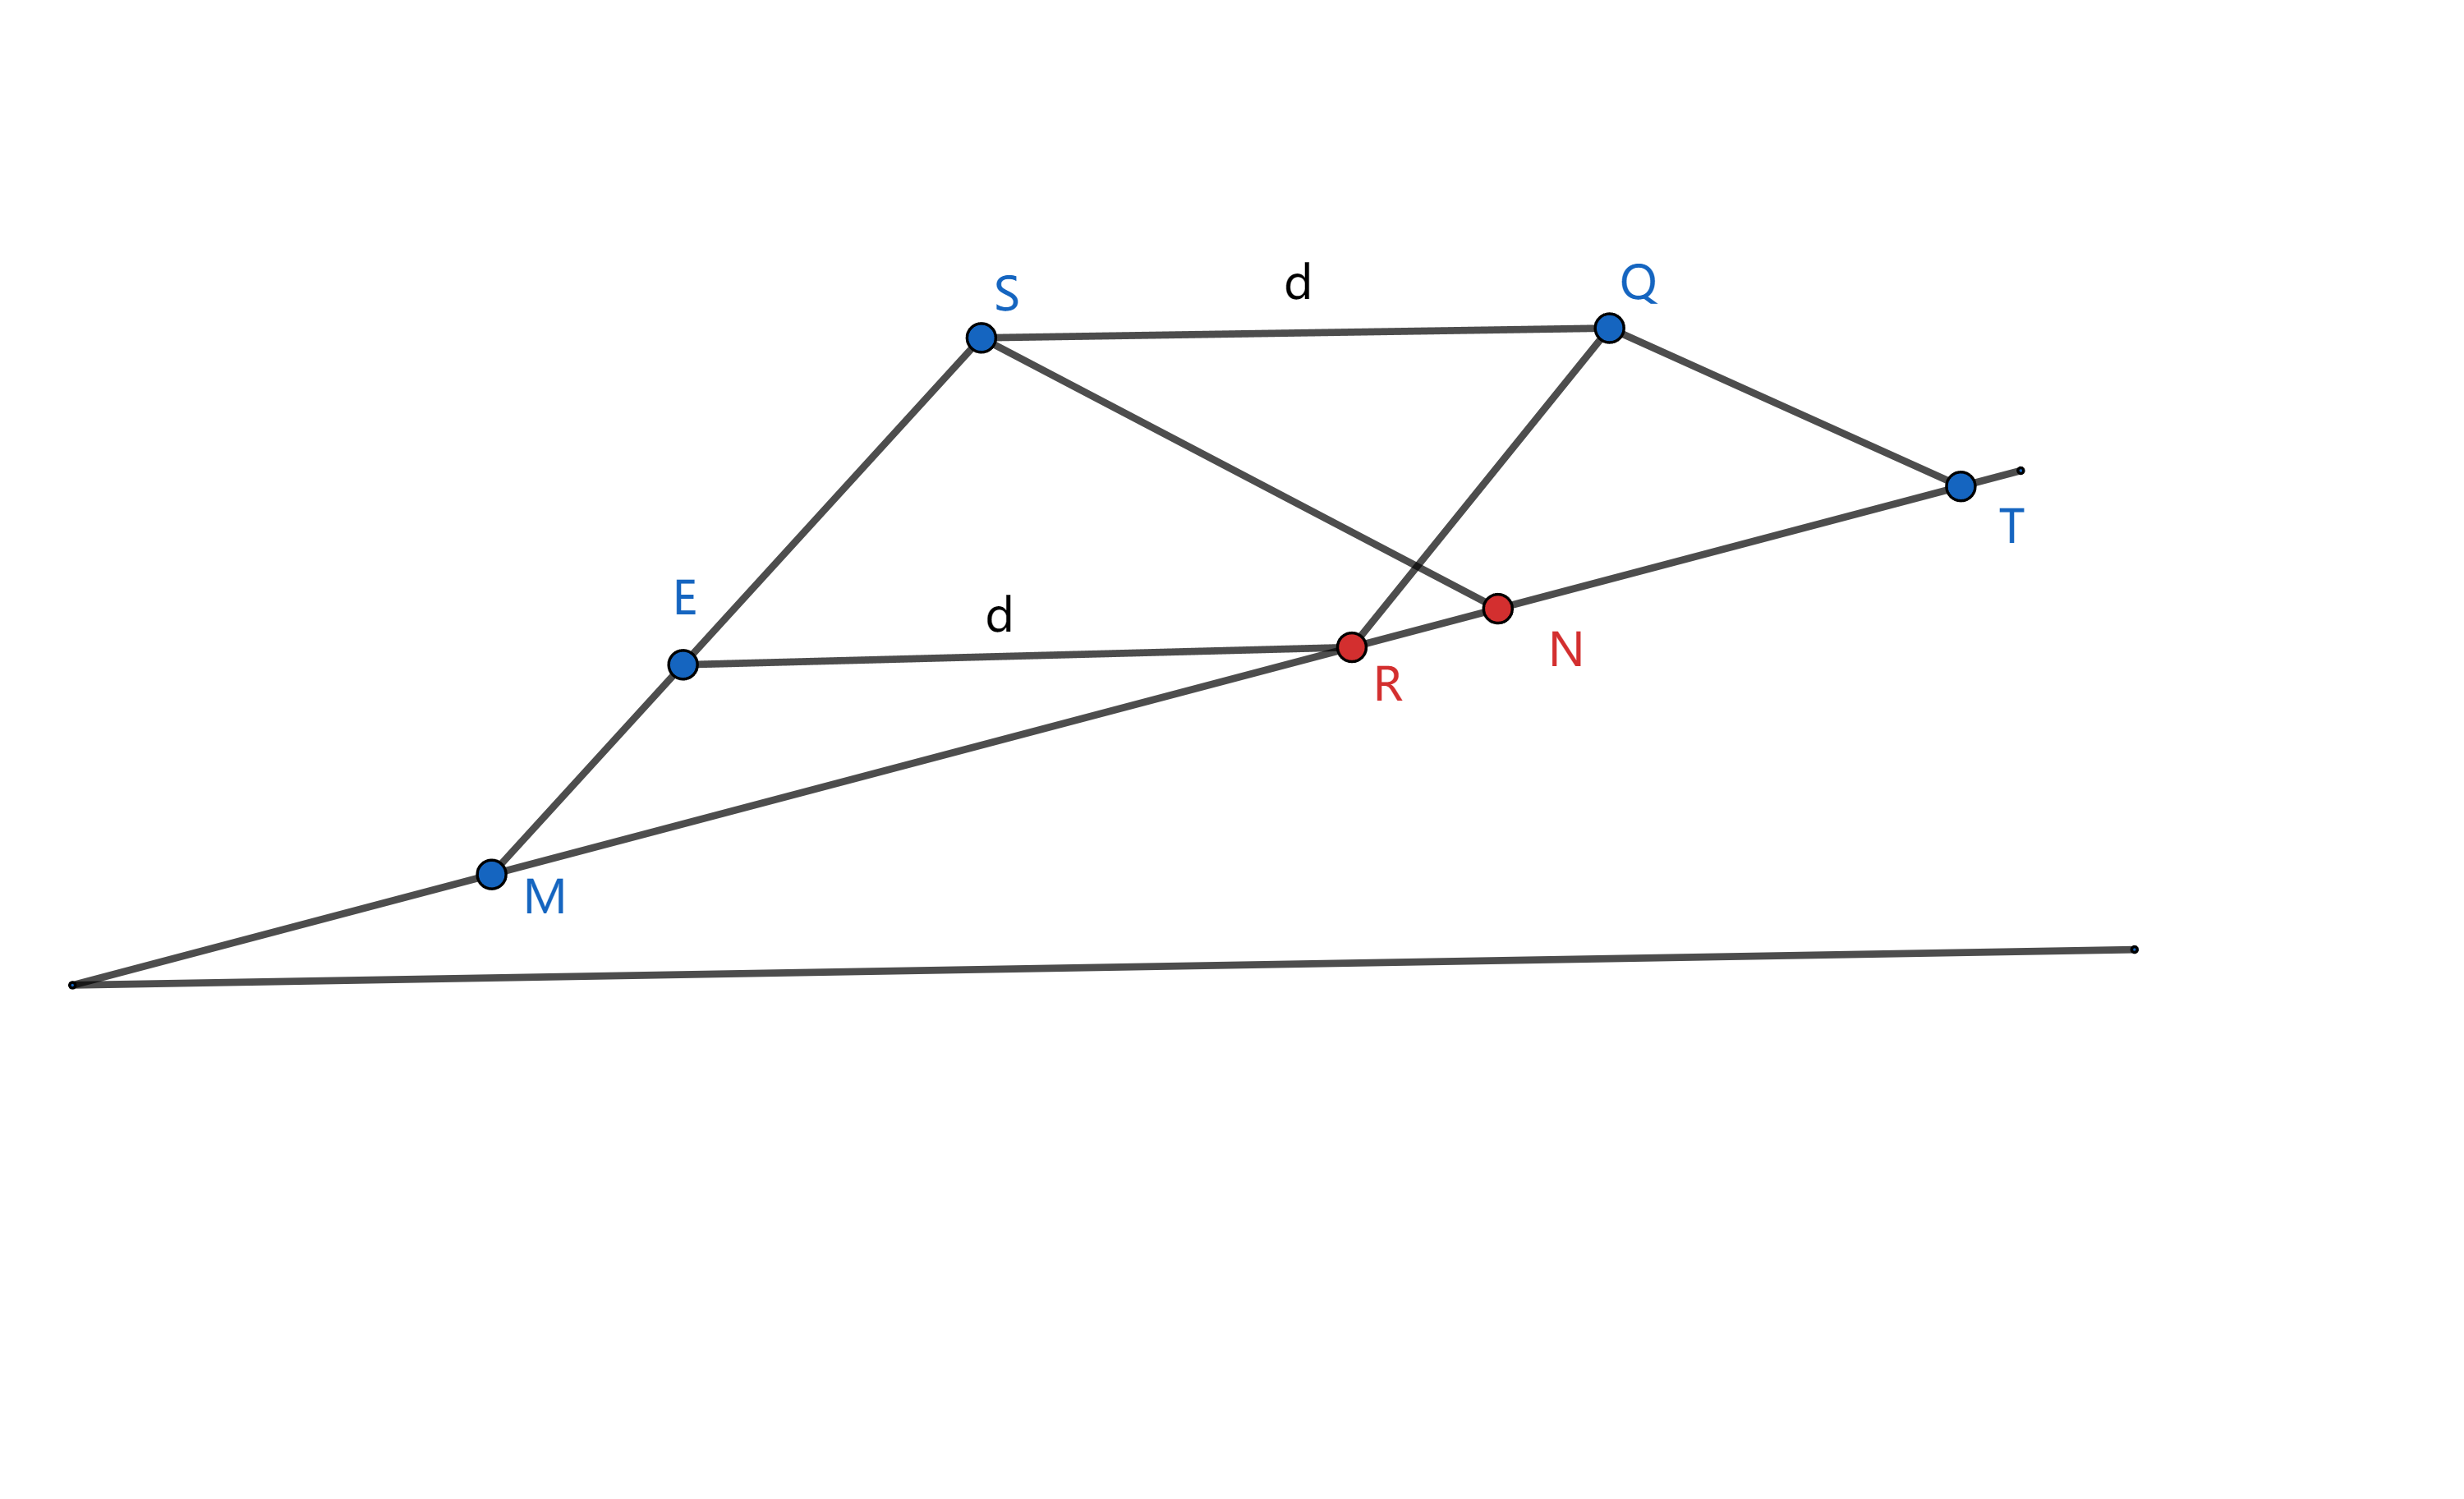
\includegraphics[width=0.95\textwidth]{问题一//问题一重叠率示意图}
		\caption{第一问重叠率的计算示意图}
		\label{pro1Eta}
	\end{figure}
	
	\par 类似题目中平坦的情况,我们把在坡度上的重叠率定义为
	\begin{equation}
	\eta = \frac{RN\cos\alpha}{w}\times 100\%=\frac{RN}{MN}\times 100\%  \label{eq4}
	\end{equation}
	其中MN可以由\eqref{eq1}和\eqref{eq2}得到,而RN的计算方式如下:
	\begin{equation}
		RN = MN - MR  \label{eq5}
	\end{equation}
	在$\Delta MER$中,由正弦定理,我们可以得到:
	\begin{equation}
		\frac{d}{\sin(\frac{\pi-\theta}{2}-\alpha)} = \frac{MR}{\sin(\frac{\pi+\theta}{2})}  \label{eq6}
	\end{equation}
	其中d是船S和船Q之间的距离,满足$d=SQ=ER$。
	\par	由\eqref{eq4}到\eqref{eq6}可以得到:
	\begin{equation}
		\eta_{i+1} = \left[ 1 - \frac{d_{i+1}\cos\frac{\theta}{2}\cos\alpha}{w_i\cos(\frac{\theta}{2}+\alpha)}\right]\times 100 \% \label{eq7}
	\end{equation}
	其中$\eta_{i+1}$是第i+1条测线相对于第i条测线(这里指更深处的测线)的重叠率,$d_{i+1}$是第i+1和第i条船的间距,$w_i$是第i条测线的覆盖宽度。
	
\subsubsection{表格一的计算结果}
	\par 题目要求计算在不同测线距中心点处距离的情况下的覆盖宽度与重叠率。设测线距中心点处距离为$S_i\in[-800,800]$,则由简单的相似关系可以得到$D_i=D_0 - S_i\sin\alpha$以及$d_i = D_i-D_{i-1}$。将$D_i$带入公式\eqref{eq3}可以得到$w_i$,将$w_i$和$d_i$带入公式\eqref{eq7}可以得到$\eta_{i}$。具体的计算结果如表\ref{ansSheet1}所示

\begin{table}[H]
	\caption{问题 1 的计算结果}\label{ansSheet1}
	\begin{tabular}{llllll}
		\hline
		测线距中心点处的距离/m  & -800     & -600        & -400         & -200         &  0\\ \hline
		海水深度/m        & 90.94156 & 85.70616898 & 80.47077932  & 75.23538966  & 70                     \\
		覆盖宽度/m        & 315.6802 & 297.506882  & 279.3335758  & 261.1602696  & 242.9869634            \\
		与前一条测线的重叠率/\% & ——       & 33.63472105 & 29.58077605  & 24.99933568  & 19.7802798             \\ \hline
		测线距中心点处的距离/m  & 200      & 400         & 600          & 800          &                        \\ \hline
		海水深度/m        & 64.76461 & 59.52922068 & 54.29383102  & 49.05844135  &                        \\
		覆盖宽度/m        & 224.8137 & 206.6403509 & 188.4670447  & 170.2937385  &                        \\
		与前一条测线的重叠率/\% & 13.78054 & 6.810804913 & -1.384863416 & -11.16109869 &                        \\ \hline
	\end{tabular}
\end{table}



\subsection{问题二:与海底坡面法向在水平面投影成一定角度时的宽度计算}
	\par 第二问的几何关系如图\ref{pro2Geo}所示:
	\begin{figure}[H]
		\centering  %图片全局居中
		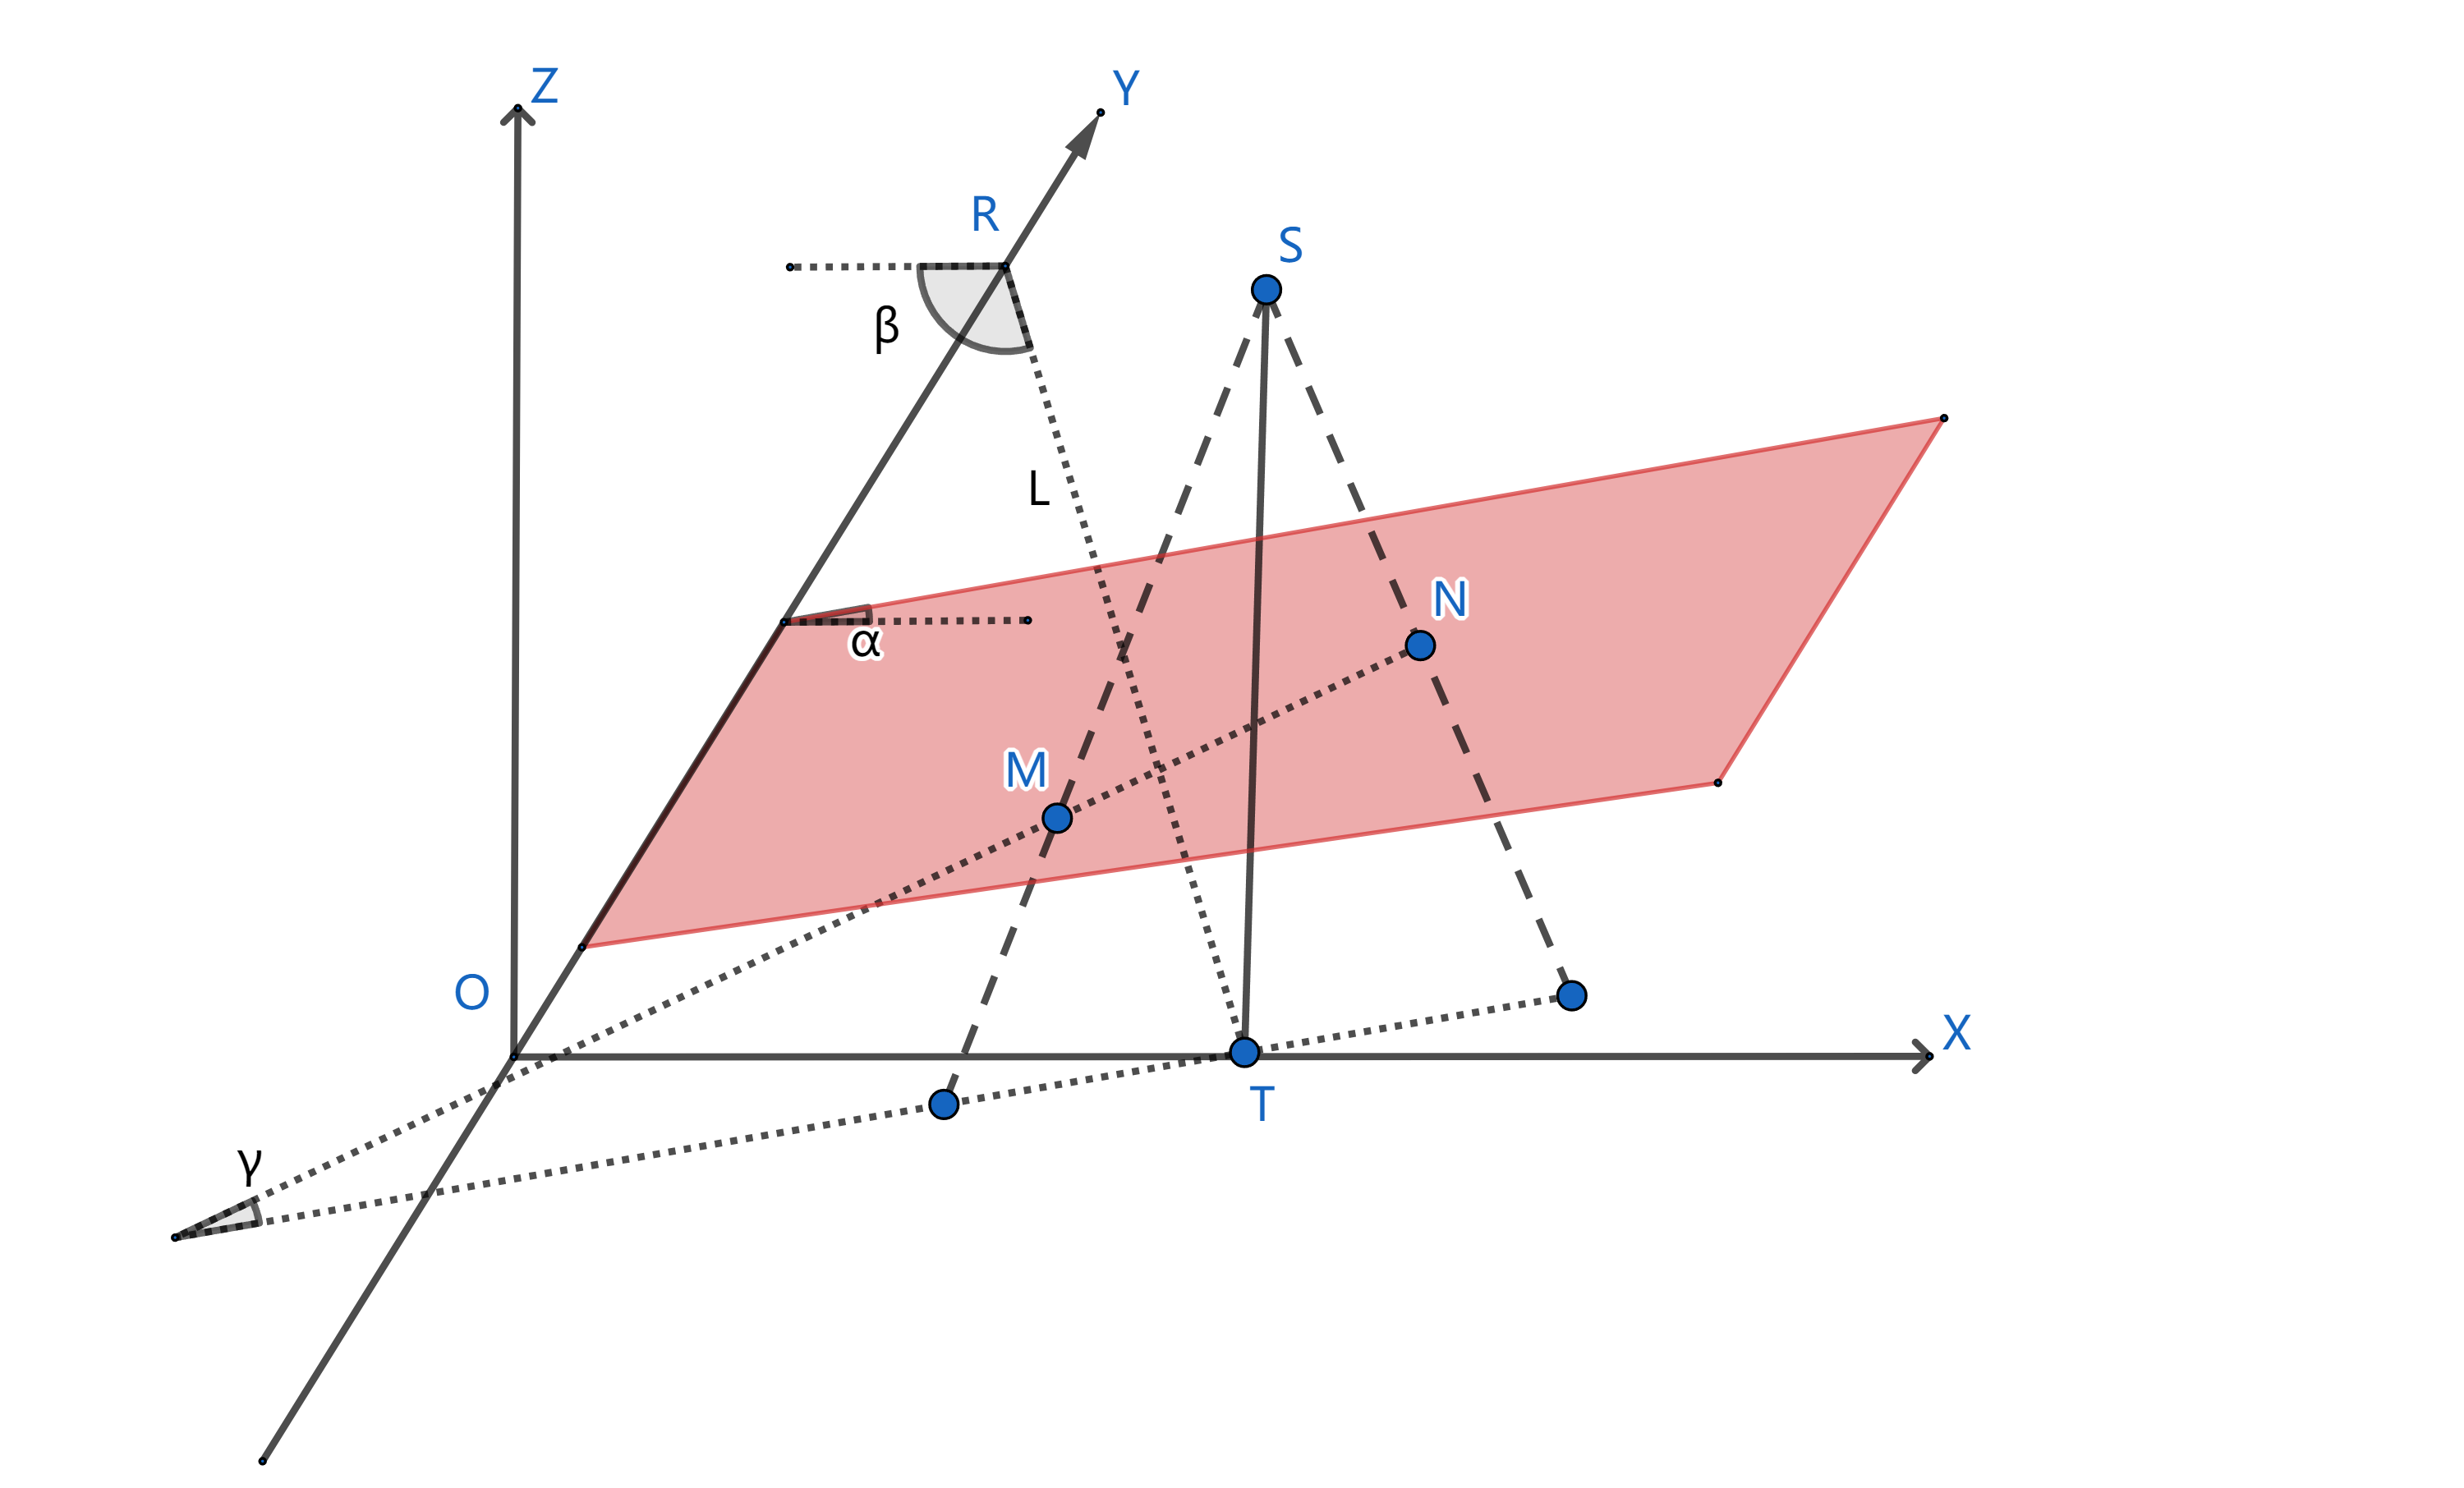
\includegraphics[width=0.95\textwidth]{问题二//第二题几何关系示意图}
		\caption{第二问几何关系示意图}
		\label{pro2Geo}
	\end{figure}
	其中S是测量船所在的位置,T是测量船位置在水平面上的投影,R是海域中心点。$w=MN\cos\gamma$是覆盖宽度,$\gamma$是$MN$与水平面形成的线面角。$L=RT$是测量船距海域中心点处的距离,$\beta$是测线方向与海底坡面的法向在水平面上投影的夹角。我们以坡面法向量在水平面上的投影方向为x方向,以等深线的方向为y方向,以竖直方向为z方向,建立如图所示的空间直角坐标系Oxyz,其中x轴经过T点,y轴经过R点。
	\par 如上文所述,第二问是第一问的延伸,只要能够求出$\gamma$,就能够变成第一问的模型。我们采用向量运算的方式来求解$\gamma$。
	\par MN所在的直线是平面SAB和海底坡面的交线。平面SAB的法向量为$v_1=[\cos\beta,\sin\beta,0]^\top$,海底坡面的法向量为$v_2=[-\sin\alpha,0,\cos\alpha]^\top$,MN直线的方向向量$v_3$需要满足:
	\begin{equation}
		v_3^\top v_1 = v_3^\top v_2 = 0  \label{eq8}
	\end{equation}
	而直线AB的方向向量可以表示为$v_4 = [\sin\beta,-\cos\beta,0]^\top$.
	\par 由于平面SAB垂直于水平面,因此有
	\begin{equation}
		\gamma = <\vec{MN},\vec{AB}> \label{eq9}
	\end{equation}
	\par 由式\eqref{eq8}\eqref{eq9}可以得到$\gamma(<\frac{\pi}{2})$的余弦值和正弦值分别为
	\begin{align}
		\cos\gamma=\frac{\cos\alpha}{\sqrt{1-\sin^2\alpha\cos^2\beta}}\\
		\sin\gamma=\frac{\sin\alpha\sin\beta}{\sqrt{1-\sin^2\alpha\cos^2\beta}}
	\end{align}
	\par 此时的覆盖宽度w的表达式为:
	\begin{align}
		w &= w(D,\beta) \notag \\
		& = D\cos\gamma\sin\frac{\theta}{2}\left[\frac{\sin\frac{\theta}{2}}{\cos(\frac{\theta}{2}+\gamma)}  +  \frac{\sin\frac{\theta}{2}}{\cos(\frac{\theta}{2}-\gamma)}\right] \notag \\
		&=D\cos\gamma\sin\frac{\theta}{2}\left[\frac{1}{\cos\frac{\theta}{2}\cos\gamma-\sin\frac{\theta}{2}\sin\gamma}  	+ \frac{1}{\cos\frac{\theta}{2}\cos\gamma+\sin\frac{\theta}{2}\sin\gamma} \right] \notag \\
		&=D\frac{\cos\alpha}{\sqrt{1-\sin^2\alpha\cos^2\beta}}\sin\frac{\theta}{2}\left[\frac{1}{\cos\frac{\theta}{2}\frac{\cos\alpha}{\sqrt{1-\sin^2\alpha\cos^2\beta}}-\sin\frac{\theta}{2}\frac{\sin\alpha\sin\beta}{\sqrt{1-\sin^2\alpha\cos^2\beta}}}  \notag	\\ &+\left. \frac{1}{\cos\frac{\theta}{2}\frac{\cos\alpha}{\sqrt{1-\sin^2\alpha\cos^2\beta}}+\sin\frac{\theta}{2}\frac{\sin\alpha\sin\beta}{\sqrt{1-\sin^2\alpha\cos^2\beta}}} \label{eq12}\right] 
	\end{align}
	注意到\textbf{w在本质上只与水深$D$和测线的方向$\beta$有关}。
	\par 当测线方向夹角为$\beta$,测量船距海域中心点处距离为$L$时,根据图\ref{pro2Geo}的几何关系,可得水深
	\begin{equation}
			D=D_0-L\sin(\beta-\frac{\pi}{2})\sin\alpha \label{13}
	\end{equation}
	其中$D_0$是海域中心点的水深。将式\eqref{13}再带入\eqref{eq12}可以得到专用于计算表2的公式:
	\begin{align}
		w&=w(L,\beta) \notag \\
		&=[D_0-L\sin(\beta-\frac{\pi}{2})\sin\alpha]\frac{\cos\alpha}{\sqrt{1-\sin^2\alpha\cos^2\beta}}\sin\frac{\theta}{2}\left[\frac{1}{\cos\frac{\theta}{2}\frac{\cos\alpha}{\sqrt{1-\sin^2\alpha\cos^2\beta}}-\sin\frac{\theta}{2}\frac{\sin\alpha\sin\beta}{\sqrt{1-\sin^2\alpha\cos^2\beta}}}  \notag	\\ &+\left.\frac{1}{\cos\frac{\theta}{2}\frac{\cos\alpha}{\sqrt{1-\sin^2\alpha\cos^2\beta}}+\sin\frac{\theta}{2}\frac{\sin\alpha\sin\beta}{\sqrt{1-\sin^2\alpha\cos^2\beta}}} \label{eq13} \right] 
	\end{align}
	\par	将表2中提供的各$\beta$与$L$值带入,取$\theta=120\degree,\, \alpha=1.5\degree,D_0=120m$,得到计算结果如下:



\begin{table}[H]
	\centering
	\caption{问题2的计算结果}
	\begin{tabular}{llllll}
		\hline
		\multicolumn{2}{l}{\multirow{2}{*}{覆盖宽度/m}} & \multicolumn{4}{l}{测量船距海域中心点处的距离/海里}      \\
		\multicolumn{2}{l}{}                        & 0        & 0.3      & 0.6      & 0.9      \\ \hline
		\multirow{8}{*}{测线方向夹角/°}       & 0         & 415.8347 & 466.2508 & 516.667  & 567.0831 \\
		& 45        & 416.1915 & 451.8717 & 487.5519 & 523.232  \\
		& 90        & 416.5491 & 416.5491 & 416.5491 & 416.5491 \\
		& 135       & 416.1915 & 380.5113 & 344.8311 & 309.151  \\
		& 180       & 415.8347 & 365.4186 & 315.0024 & 264.5863 \\
		& 225       & 416.1915 & 380.5113 & 344.8311 & 309.151  \\
		& 270       & 416.5491 & 416.5491 & 416.5491 & 416.5491 \\
		& 315       & 416.1915 & 451.8717 & 487.5519 & 523.232  \\ \hline
		\multicolumn{2}{l}{\multirow{2}{*}{覆盖宽度/m}} & \multicolumn{4}{l}{测量船距海域中心点处的距离/海里}      \\
		\multicolumn{2}{l}{}                        & 1.2      & 1.5      & 1.8      & 2.1      \\ \hline
		\multirow{8}{*}{测线方向夹角/°}       & 0         & 617.4992 & 667.9154 & 718.3315 & 768.7477 \\
		& 45        & 558.9122 & 594.5924 & 630.2726 & 665.9528 \\
		& 90        & 416.5491 & 416.5491 & 416.5491 & 416.5491 \\
		& 135       & 273.4708 & 237.7906 & 202.1104 & 166.4302 \\
		& 180       & 214.1701 & 163.754  & 113.3379 & 62.92173 \\
		& 225       & 273.4708 & 237.7906 & 202.1104 & 166.4302 \\
		& 270       & 416.5491 & 416.5491 & 416.5491 & 416.5491 \\
		& 315       & 558.9122 & 594.5924 & 630.2726 & 665.9528 \\ \hline
	\end{tabular}
\end{table}
	

	




\subsection{问题三:矩形理想海域内最短布线规划}
\subsection{问题四:真实海域内多目标最优布线规划}

\section{模型优缺点评价}

\section*{参考文献}
% \bibliographystyle{unsrt}
% \bibliography{ref.bib}
	
	
\section*{附录}
	
	
	
	
	
%\begin{figure}[H]
%	\centering  %图片全局居中
%	\subfigure[步长h=0.01]{
%		\label{exEuler.sub.1}
%		\includegraphics[width=0.45\textwidth]{各种方法的轨道形态对比//平面上的单体问题,显式欧拉法,步长=0.01,时间范围:0~100}}
%	\subfigure[步长h=0.001]{
%		\label{exEulr.sub.2}
%		\includegraphics[width=0.45\textwidth]{各种方法的轨道形态对比//平面上的单体问题,显式欧拉法,步长=0.001,时间范围:0~100}}
%	\caption{显式欧拉法}
%	\label{exEuler.main}
%\end{figure}



\end{document}